\documentclass[12pt,a4paper]{article}
\usepackage{amssymb}
\usepackage{fullpage}
\usepackage{graphicx}
\author{Parker Whaley}
\title{lab \#4}
\begin{document}
\maketitle
\section{tabulation of data}
Note that the uncertainty in all measurements is $\delta=.0005m$ unless otherwise noted.
\subsection{different radii of the lens}
The detentions of the masks in meters and there focal positions (yellow light).  For this our object was located at .1235m and our lens was at .693m\\
\begin{tabular}{|l|l|l|l|l|}
\hline
$R_i$ & $R_o$ & $R_{ave}$ & $\delta R_{ave}$ & image\\
\hline
.013 & .018 & .0155 & .0025&1.0765\\ \hline
.018 & .0225& .02025 & .00225&1.0720\\ \hline
.0225 & .0295& .026& .0035&1.0660\\ \hline
.02875 & .03425& .0315& .00275&1.0575\\ \hline
.035 & .0395& .03725& .00225&1.0500\\ \hline
.039 & .042 & .0405 & .0015&1.0415\\ \hline
.0415 & .0455& .0435& .002&1.0340\\ \hline
.0445 & .0495& .047& .0025&1.0270\\ \hline
.0495 & .053 & .05125& .00175&1.0180\\ \hline
.05325 & .0565 & .054875& .001625&1.0130\\ \hline
.05625 & .05875 & .0575& .00125&1.0010\\ \hline
\end{tabular}
\subsection{chromatic aberration}
Firstly we have our spectra for the different filters:\\
\begin{tabular}{c c c}
yellow & red & orange\\
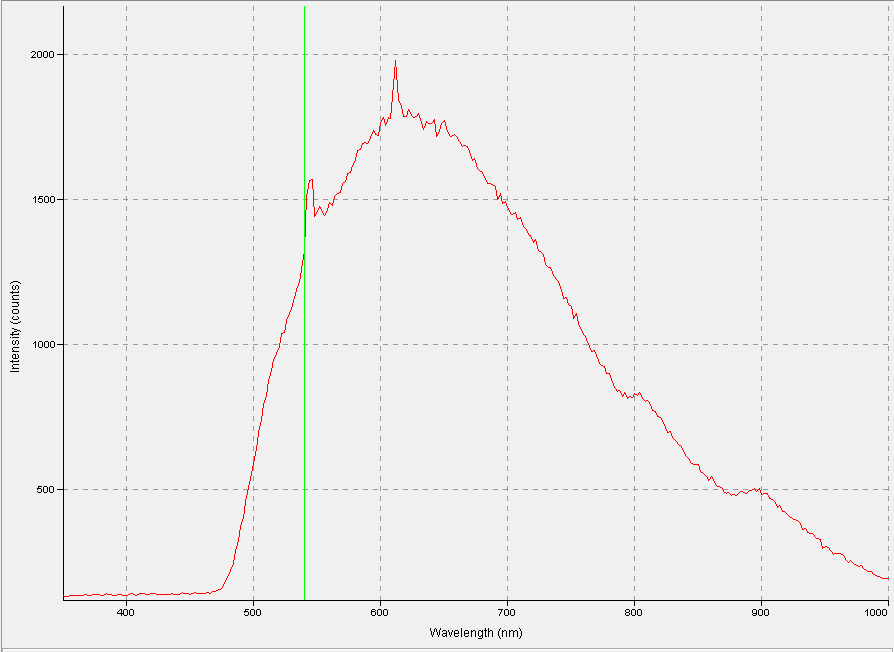
\includegraphics[scale=.23]{yellow} & 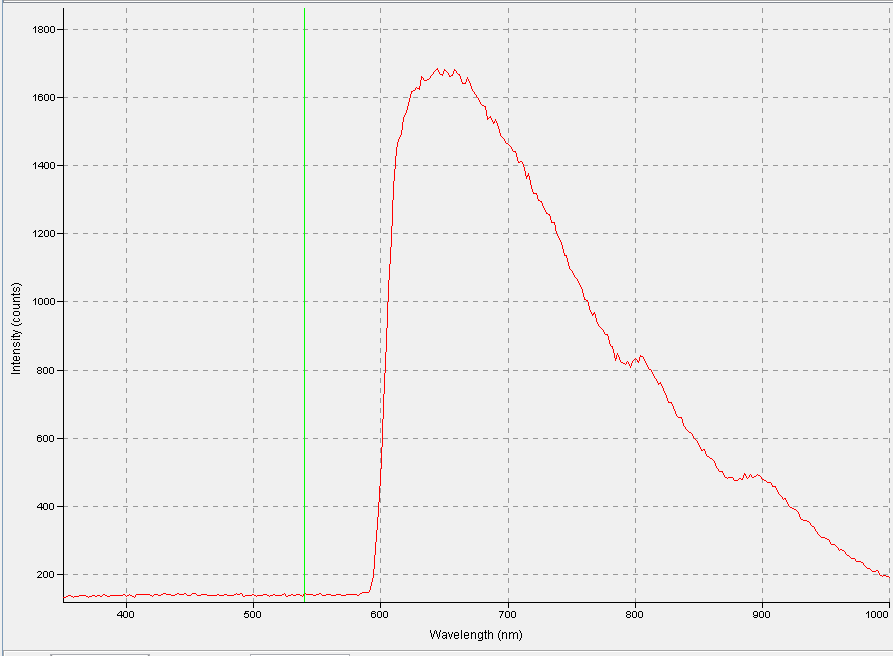
\includegraphics[scale=.23]{red} & 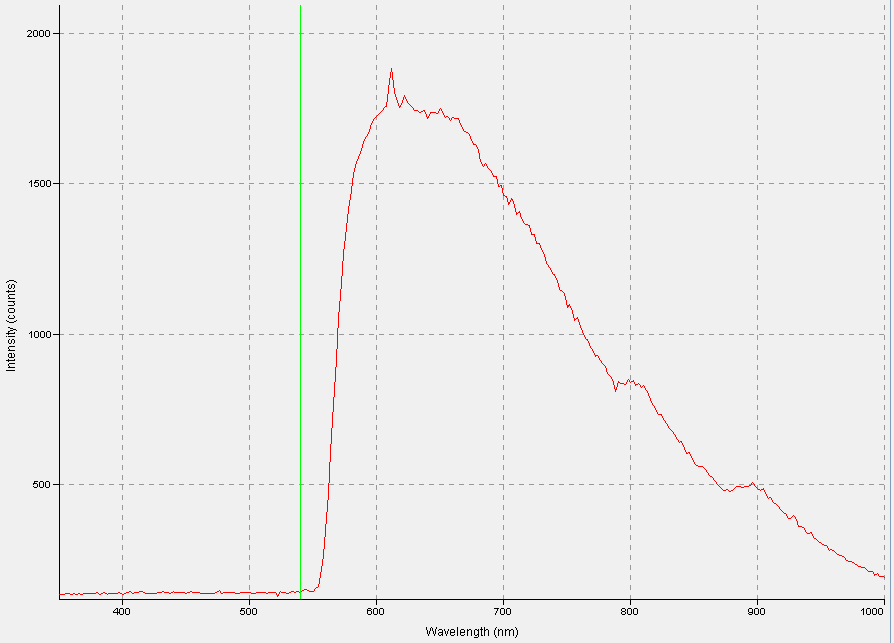
\includegraphics[scale=.23]{orange}\\
green & blue & violet\\
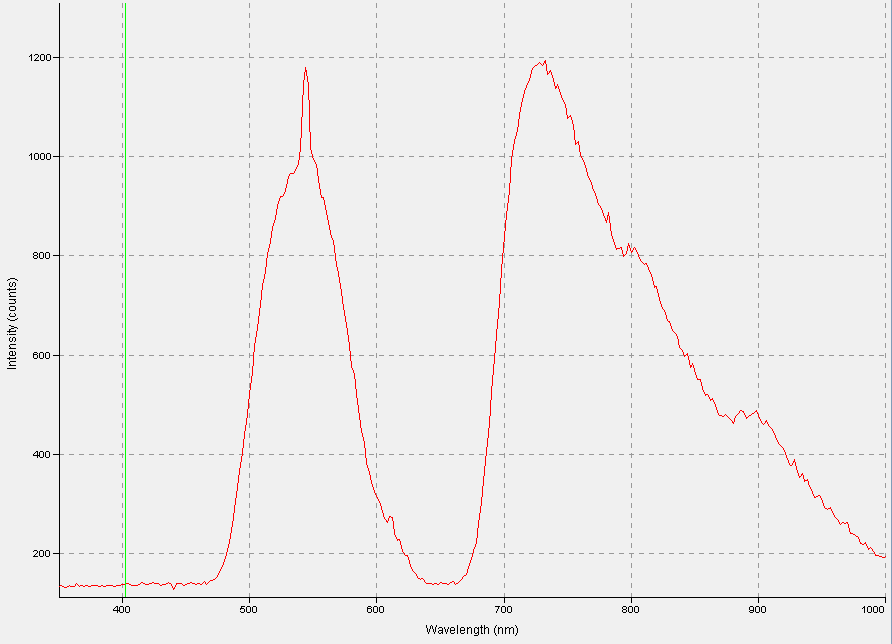
\includegraphics[scale=.23]{green} & 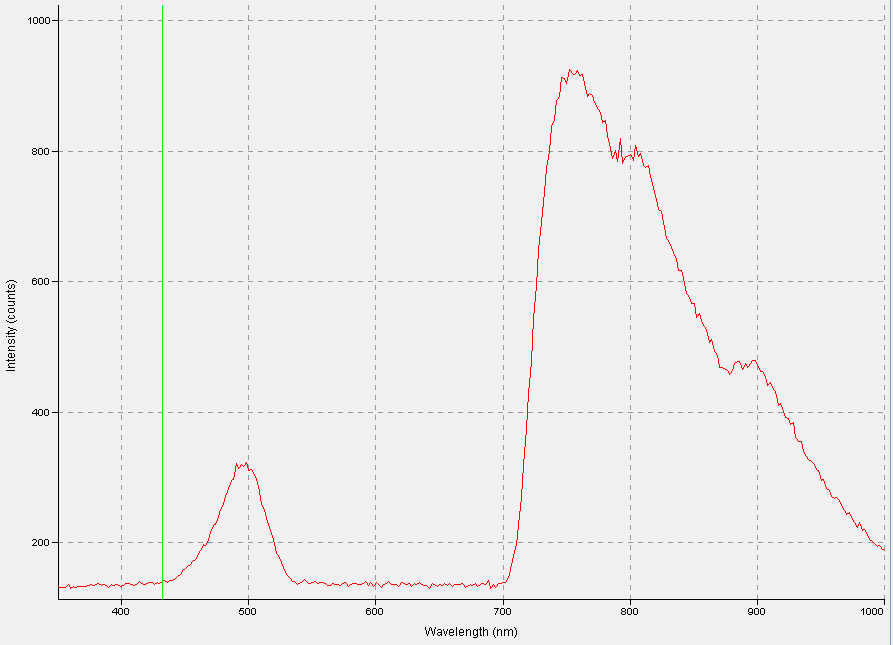
\includegraphics[scale=.23]{blue} & 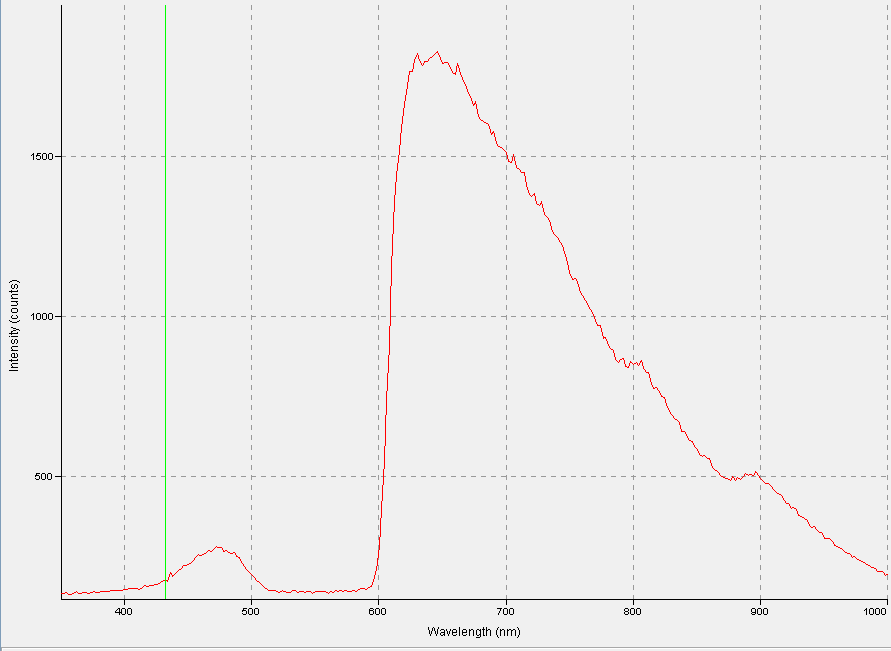
\includegraphics[scale=.23]{violet}\\
\end{tabular}
For this our object was located at .1235m and our lens was at .8055m.  The uncertainty in the wavelength is high since they are very spread out so $\delta \lambda=15nm$\\
\begin{tabular}{|l|l|l|}
\hline
color & image (m) & wavelength (nm)\\
\hline
yellow & 1.1965 & 625\\
\hline
red & 1.1985 & 650\\
\hline
orange & 1.1985 & 615\\
\hline
green & 1.1915 & 550\\
\hline
blue & 1.187 & 500\\
\hline
violet & 1.186 & 475\\
\hline
\end{tabular}
\subsection{sagital and tangential aberration}
For this our object was located at .1235m and our lens was at .92m.\\
\begin{tabular}{|l|l|l|}
\hline
angle & sagital image (m) & tangential image (m)\\
\hline
-35 & 1.151 & 1.334\\
\hline
-30 & 1.204 & 1.3565\\
\hline
-25 & 1.269 & 1.364\\
\hline
-20 & 1.312 & 1.379\\
\hline
-15 & 1.353 & 1.386\\
\hline
-10 & 1.3775 & 1.397\\
\hline
10 & 1.376 & 1.395\\
\hline
15 & 1.351 & 1.386\\
\hline
20 & 1.315 & 1.3675\\
\hline
25 & 1.268 & 1.3565\\
\hline
30 & 1.201 & 1.328\\
\hline
35 & 1.155 & 1.323\\
\hline

\end{tabular}

\section{analysis}
Here we see a significant inverse relationship between the focal length and the diameter of the mask.\\
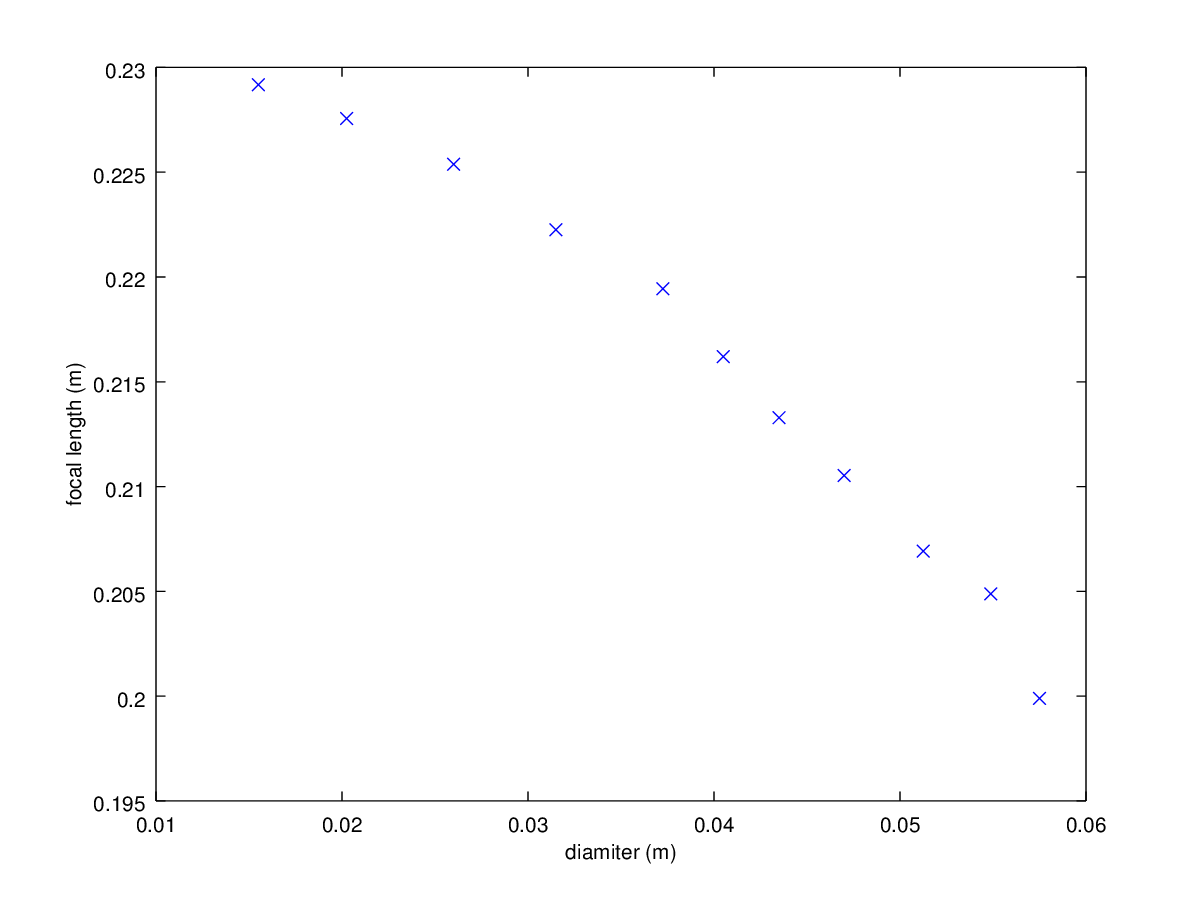
\includegraphics[scale=.7]{diamvsf}\\
This is the focal length for various colors.\\
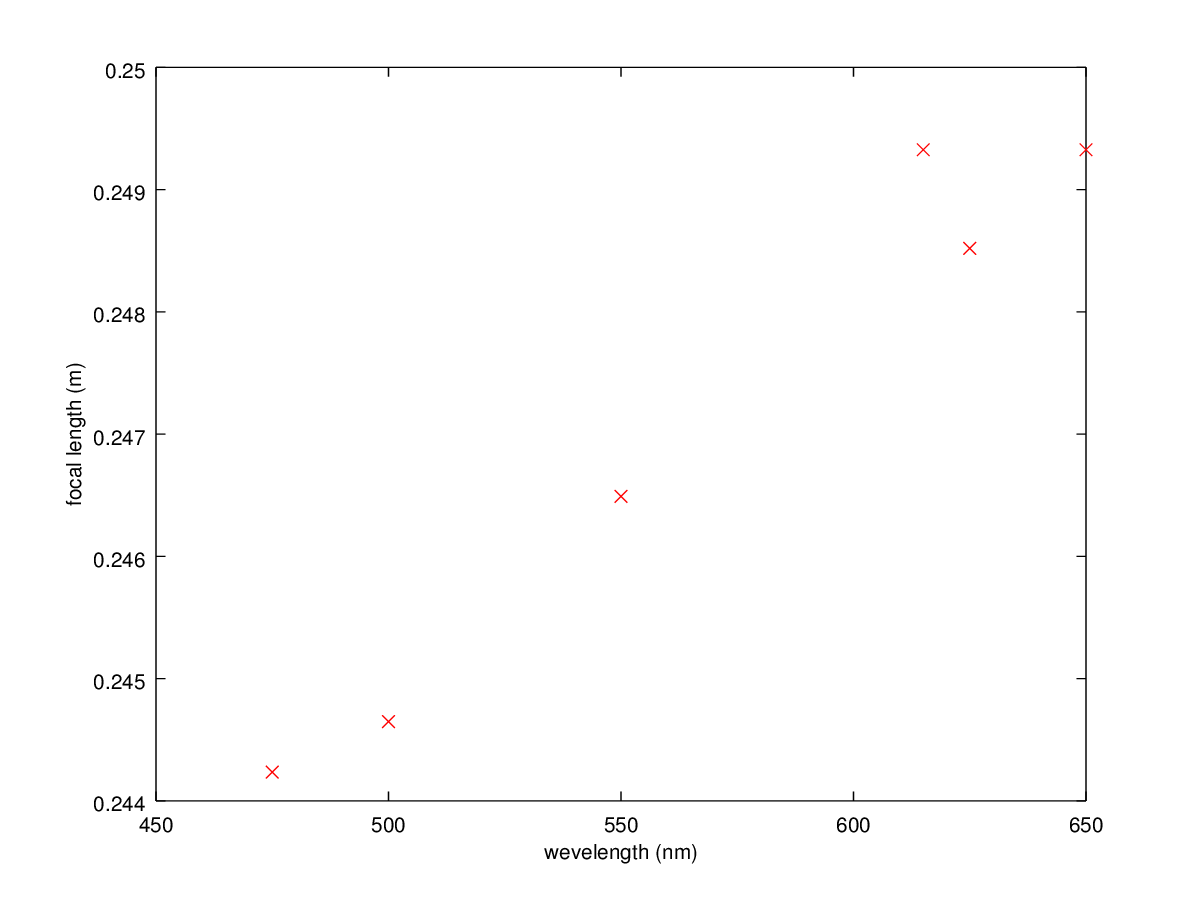
\includegraphics[scale=.7]{wevevsf}\\
This is a plot of the sagital and tangential focal lengths vs the angle of rotation.\\
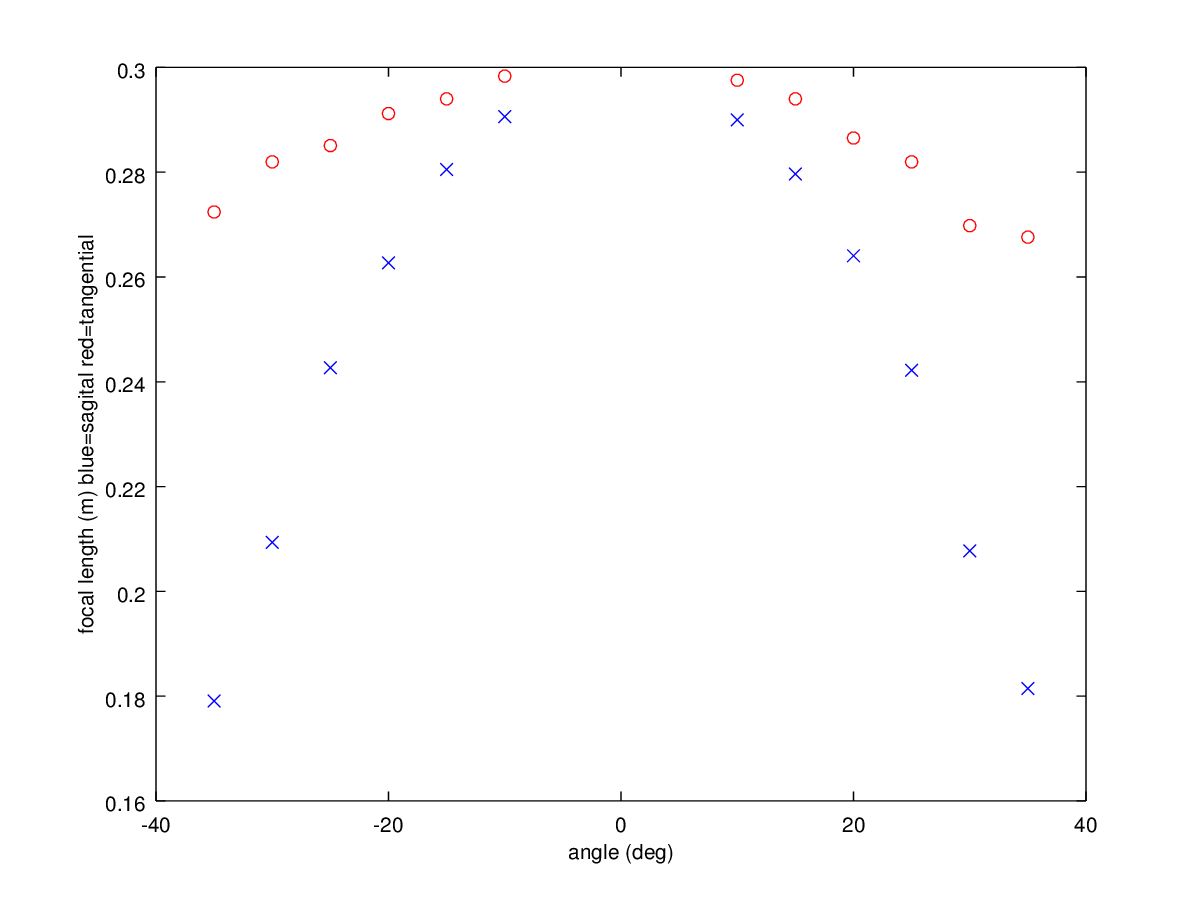
\includegraphics[scale=.7]{sandt}\\
\section{additional discussion}
The spherical aberration we observed seams to be consistent with the inverse relationship described in the book.  The rays passing through the higher radius regions seem to be bent in more, as expected.\\

Since glass has a higher reflective index for smaller wavelength light we would expect that the lens (who's effect is proportional to the reflective index) would be stronger for smaller wavelengths.  This is the result shown in the above graph.\\



\end{document}